\documentclass[12pt,a4paper]{article}
\usepackage[T2A]{fontenc}
\usepackage[utf8]{inputenc}
\usepackage[russian]{babel}
\usepackage{amsmath, amssymb}
\usepackage{geometry}
\usepackage{booktabs}
\usepackage{array}
\usepackage{graphicx}
\usepackage{hyperref}
\hypersetup{hidelinks}
\usepackage{xcolor}
\usepackage{listings}
\usepackage{caption}
\usepackage{float}

\geometry{left=2.5cm, right=2cm, top=2cm, bottom=2cm}
\graphicspath{{figures/}}

\lstset{
  basicstyle=\small\ttfamily,
  backgroundcolor=\color{gray!10},
  frame=single,
  breaklines=true,
  inputencoding=utf8,
  extendedchars=true
}

\title{\textbf{Домашнее задание №1 и №2}\\
\large Методы оптимизации: кубическая аппроксимация и безусловная оптимизация функции двух переменных\\[0.5em]
\normalsize ИТМО, 2 курс, 4 семестр}
\author{%
  Вариант 9\\[0.4em]
  Студенты: Калинин Дмитрий, Рзаев Ахмед\\
  Преподаватель: Селина Е.\,Г.
}
\date{}

\begin{document}
\maketitle
\tableofcontents
\newpage

\section{Исходные данные и состав работы}

Выполнены все пункты первых двух блоков домашнего задания:
\begin{itemize}
  \item ДЗ1.1 из файла \texttt{ЛР3.pdf}: метод кубической аппроксимации для функции одной переменной;
  \item ДЗ1.2 из файла \texttt{ЛР3.pdf}: визуализация исходной и аппроксимирующей функций;
  \item ДЗ2.1 из файла \texttt{ЛР4.pdf}: линии уровня и траектории трех методов из ЛР4;
  \item ДЗ2.2 из файла \texttt{ЛР4.pdf}: метод Ньютона и аналитическая классификация стационарных точек;
  \item ДЗ2.3 из файла \texttt{ЛР4.pdf}: объектная модель трех методов оптимизации.
\end{itemize}

Расчеты разнесены по отдельным простым программам:
\begin{itemize}
  \item \texttt{dz1\_1\_cubic\_approximation.py} --- численный метод кубической аппроксимации;
  \item \texttt{dz1\_2\_visualization.py} --- графики исходной функции и кубических аппроксимаций;
  \item \texttt{dz2\_1\_contours.py} --- линии уровня и траектории трех методов;
  \item \texttt{dz2\_2\_newton.py} --- метод Ньютона и классификация стационарных точек;
  \item \texttt{dz2\_3\_object\_model.py} --- объектная модель и ООП-реализация методов.
\end{itemize}
Файл \texttt{homework.py} оставлен как общий запускатель всех программ. Сводка результатов сохранена в \texttt{build/results.json}.

\section{ДЗ №1.1. Метод кубической аппроксимации}

\subsection{Постановка задачи}

Для варианта 9 задана функция
\begin{equation}
  f(x) = \frac{x^3}{3} - 5x + x\ln x, \qquad [a,b]=[1.5,2].
\end{equation}

Производные:
\begin{equation}
  f'(x)=x^2+\ln x-4, \qquad f''(x)=2x+\frac{1}{x}.
\end{equation}

На рассматриваемом отрезке $f''(x)>0$, следовательно функция выпукла и имеет единственный минимум. Проверка знаков производной на концах:
\begin{equation}
  f'(1.5)=-1.344535 < 0, \qquad f'(2)=0.693147 > 0.
\end{equation}

Значит точка минимума лежит внутри отрезка.

\subsection{Формулы метода}

На каждой итерации строится кубический интерполяционный многочлен Эрмита по значениям $f(u)$, $f(v)$ и производным $f'(u)$, $f'(v)$ на текущем отрезке $[u,v]$. Для нахождения стационарной точки кубики использовались формулы:

Для вывода формул удобно обозначать текущие границы отрезка как $u$ и $v$, чтобы не путать их с коэффициентами кубического многочлена. Пусть
\begin{equation}
  h=v-u.
\end{equation}
Кубическую аппроксимацию можно записать в локальной форме:
\begin{equation}
  m(x)=f(u)+f'(u)(x-u)+b_k(x-u)^2+a_k(x-u)^3.
\end{equation}
Здесь $a_k$ и $b_k$ --- коэффициенты кубической модели на $k$-й итерации. Они находятся из двух условий согласования в правом конце отрезка:
\begin{equation}
  m(v)=f(v), \qquad m'(v)=f'(v).
\end{equation}
Введем вспомогательные величины:
\begin{equation}
  A_k=f(v)-f(u)-f'(u)h, \qquad B_k=f'(v)-f'(u).
\end{equation}
Тогда из системы
\begin{equation}
  a_kh^3+b_kh^2=A_k, \qquad 3a_kh^2+2b_kh=B_k
\end{equation}
получаются коэффициенты:
\begin{equation}
  a_k=\frac{B_kh-2A_k}{h^3}, \qquad
  b_k=\frac{3A_k-B_kh}{h^2}.
\end{equation}

Чтобы найти минимум кубической аппроксимации, решается уравнение $m'(x)=0$:
\begin{equation}
  m'(x)=f'(u)+2b_k(x-u)+3a_k(x-u)^2=0.
\end{equation}
Если положить $y=x-u$, то получается квадратное уравнение
\begin{equation}
  3a_ky^2+2b_ky+f'(u)=0.
\end{equation}
Его корни:
\begin{equation}
  y=\frac{-b_k\pm\sqrt{b_k^2-3a_kf'(u)}}{3a_k}.
\end{equation}
Из двух корней выбирается тот, который попадает в текущий отрезок: $0\le y\le h$, после чего $x^*=u+y$. В программе использована эквивалентная компактная запись через величины $w$ и $z$:
\begin{equation}
  w = f'(v)+f'(u)-3\frac{f(v)-f(u)}{v-u},
\end{equation}
\begin{equation}
  z = \sqrt{w^2-f'(u)f'(v)},
\end{equation}
\begin{equation}
  x^* = v - (v-u)\frac{f'(v)+z-w}{f'(v)-f'(u)+2z}.
\end{equation}

Для первой итерации:
\begin{equation}
  x_1=1.5,\qquad x_2=2,\qquad h=x_2-x_1=0.5.
\end{equation}
Значения функции и производной на концах:
\begin{equation}
  f(1.5)=-5.766802,\qquad f(2)=-5.947039,
\end{equation}
\begin{equation}
  f'(1.5)=-1.344535,\qquad f'(2)=0.693147.
\end{equation}
В обозначениях метода Дэвидона:
\begin{equation}
  z_1=\frac{3(f(x_1)-f(x_2))}{x_2-x_1}+f'(x_1)+f'(x_2)
  =0.430032,
\end{equation}
\begin{equation}
  w_1=\sqrt{z_1^2-f'(x_1)f'(x_2)}
  =1.056829.
\end{equation}
Коэффициент шага:
\begin{equation}
  \mu_1=\frac{f'(x_2)+w_1-z_1}{f'(x_2)-f'(x_1)+2w_1}
  =0.317956.
\end{equation}
Новая точка:
\begin{equation}
  \overline{x}_1=x_2-\mu_1(x_2-x_1)
  =2-0.317956\cdot 0.5=1.841022.
\end{equation}
Так как $f'(1.841022)\approx -3.175\cdot 10^{-4}<0$, минимум расположен правее этой точки, поэтому новый отрезок:
\begin{equation}
  [1.841022,\;2].
\end{equation}

Для визуализации кубическую аппроксимацию можно также записывать в обычном виде
\begin{equation}
  P(x)=ax^3+bx^2+cx+d.
\end{equation}
Коэффициенты $a,b,c,d$ находятся из условий совпадения значений функции и производных на концах отрезка:
\begin{equation}
\begin{cases}
  ax_1^3+bx_1^2+cx_1+d=f(x_1),\\
  ax_2^3+bx_2^2+cx_2+d=f(x_2),\\
  3ax_1^2+2bx_1+c=f'(x_1),\\
  3ax_2^2+2bx_2+c=f'(x_2).
\end{cases}
\end{equation}
Для первой итерации матричная система имеет вид:
\begin{equation}
\begin{pmatrix}
1.5^3 & 1.5^2 & 1.5 & 1\\
2^3 & 2^2 & 2 & 1\\
3\cdot 1.5^2 & 2\cdot 1.5 & 1 & 0\\
3\cdot 2^2 & 2\cdot 2 & 1 & 0
\end{pmatrix}
\begin{pmatrix}
a\\b\\c\\d
\end{pmatrix}
=
\begin{pmatrix}
-5.766802\\
-5.947039\\
-1.344535\\
0.693147
\end{pmatrix}.
\end{equation}
Решение системы:
\begin{equation}
  a=0.278235,\qquad b=0.576947,\qquad c=-4.953463,\qquad d=-0.573782.
\end{equation}
Следовательно, кубическая аппроксимация первой итерации:
\begin{equation}
  P_1(x)=0.278235x^3+0.576947x^2-4.953463x-0.573782.
\end{equation}

Правило обновления отрезка:
\begin{equation}
  \begin{cases}
    v := x^*, & f'(x^*)>0,\\
    u := x^*, & f'(x^*)<0.
  \end{cases}
\end{equation}
Критерий останова: $|f'(x^*)|<\varepsilon$, где $\varepsilon=10^{-4}$.

\begin{table}[H]
\centering
\caption{Коэффициенты кубической модели на итерациях}
\begin{tabular}{cccccc}
\toprule
$k$ & $u$ & $v$ & $h$ & $a_k$ & $b_k$ \\
\midrule
1 & 1.500000 & 2.000000 & 0.500000 & 0.278235 & 1.829006 \\
2 & 1.841022 & 2.000000 & 0.158978 & 0.288100 & 2.112305 \\
\bottomrule
\end{tabular}
\end{table}

\subsection{Итерации}

\begin{table}[H]
\centering
\caption{Итерации метода кубической аппроксимации}
\begin{tabular}{cccccc}
\toprule
$k$ & $u$ & $v$ & $f'(u)$ & $f'(v)$ & $x^*$ \\
\midrule
1 & 1.500000 & 2.000000 & -1.344535 & 0.693147 & 1.841022 \\
2 & 1.841022 & 2.000000 & -0.000318 & 0.693147 & 1.841097 \\
\bottomrule
\end{tabular}
\end{table}

\begin{table}[H]
\centering
\caption{Контроль точности на итерациях}
\begin{tabular}{ccccc}
\toprule
$k$ & $f(x^*)$ & $f'(x^*)$ & $|f'(x^*)|$ & длина отрезка \\
\midrule
1 & -6.001532545 & $-3.175053\cdot 10^{-4}$ & $3.175053\cdot 10^{-4}$ & 0.500000 \\
2 & -6.001532557 & $4.582998\cdot 10^{-8}$ & $4.582998\cdot 10^{-8}$ & 0.158978 \\
\bottomrule
\end{tabular}
\end{table}

Итог:
\begin{equation}
  \boxed{x_{\min}\approx 1.841097}, \qquad
  \boxed{f(x_{\min})\approx -6.001533}.
\end{equation}

Критерий выполнен, так как $|f'(x^*)|=4.58\cdot 10^{-8}<10^{-4}$.

\section{ДЗ №1.2. Визуализация исходной и аппроксимирующей функций}

По условию ДЗ1.2 нужно программно построить исходную функцию и аппроксимирующие функции в одной координатной плоскости для итераций алгоритма. Для каждой итерации построена кубическая модель Эрмита на текущем отрезке $[u,v]$.

\begin{figure}[H]
  \centering
  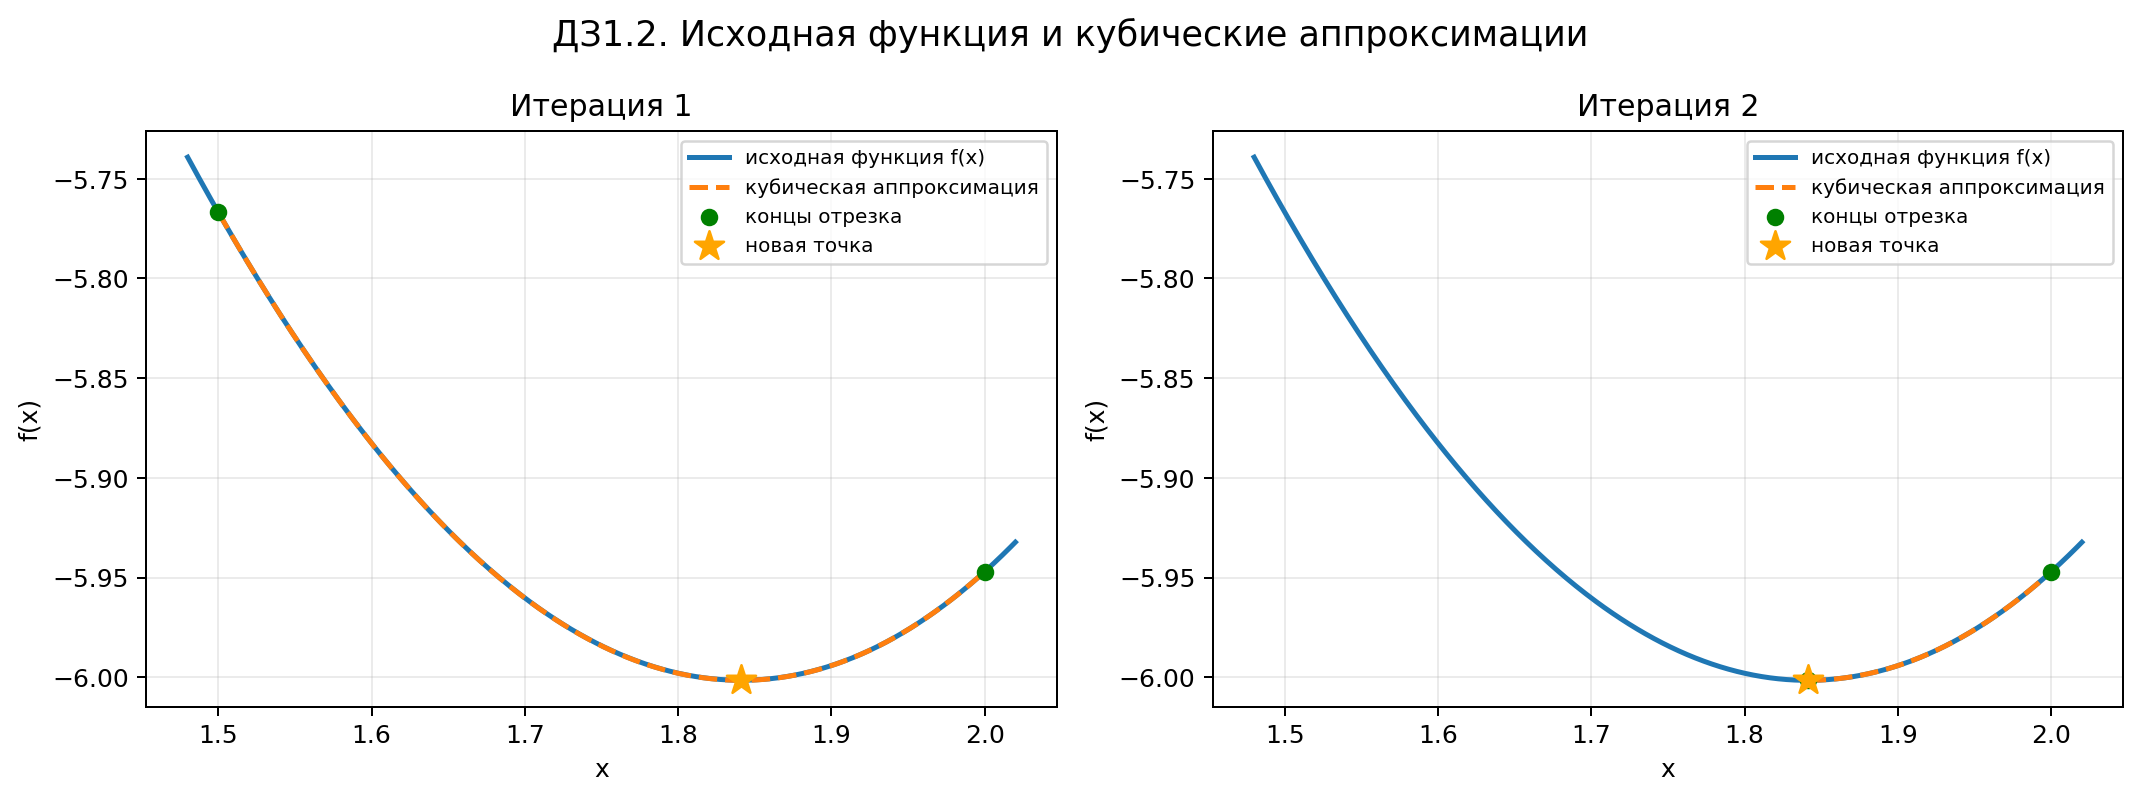
\includegraphics[width=\textwidth]{dz1_cubic_iterations.png}
  \caption{Исходная функция и кубические аппроксимации на итерациях метода.}
\end{figure}

\begin{figure}[H]
  \centering
  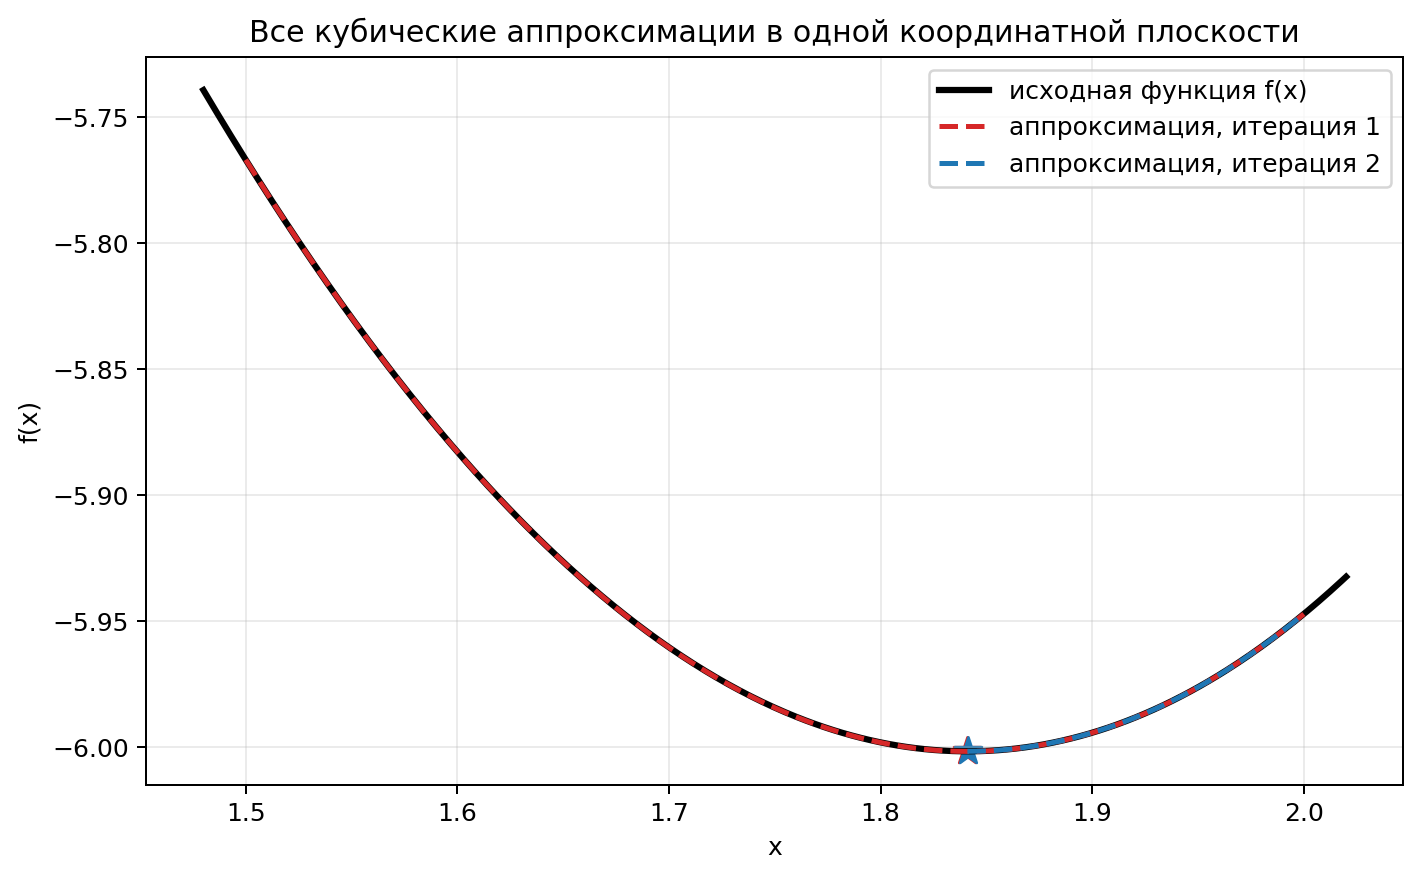
\includegraphics[width=0.82\textwidth]{dz1_cubic_all_approximations.png}
  \caption{Исходная функция и все кубические аппроксимации в одной координатной плоскости.}
\end{figure}

\begin{figure}[H]
  \centering
  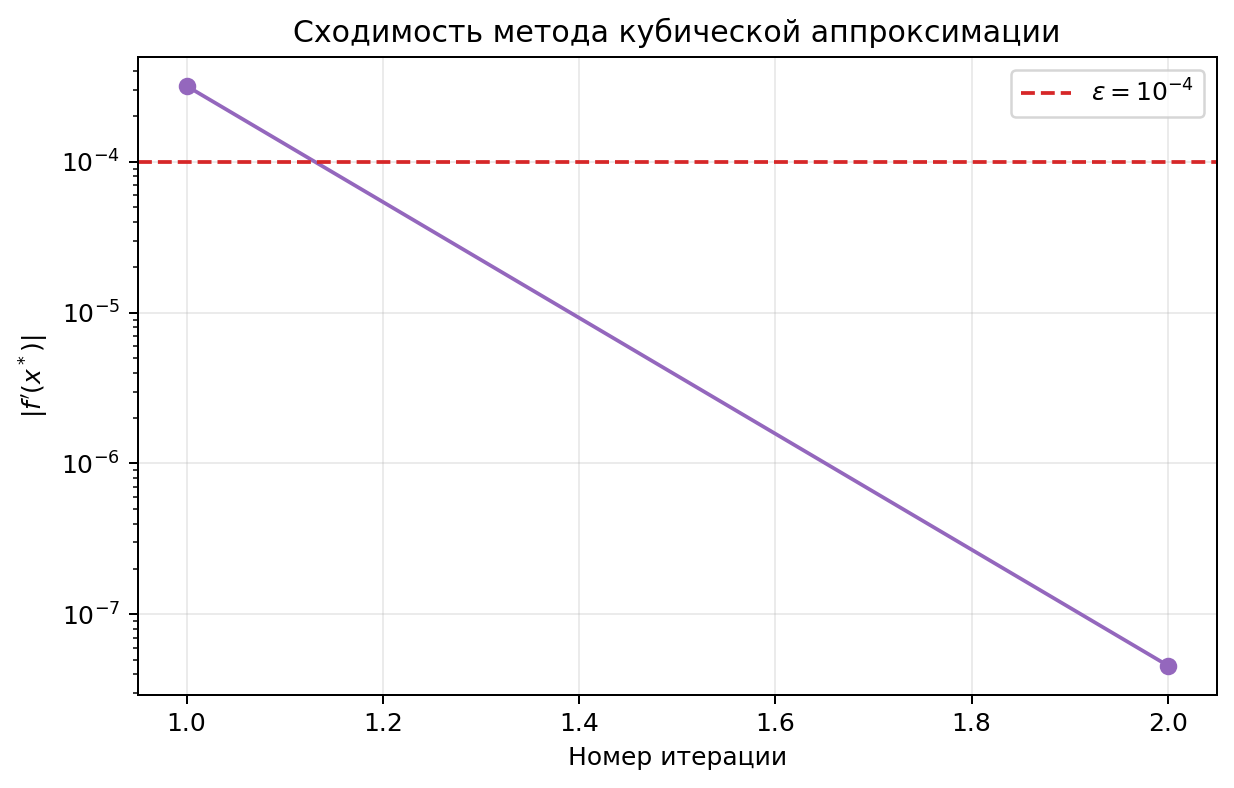
\includegraphics[width=0.75\textwidth]{dz1_cubic_convergence.png}
  \caption{Сходимость метода по величине $|f'(x^*)|$.}
\end{figure}

\section{ДЗ №2.1. Линии уровня и траектории методов ЛР4}

\subsection{Постановка задачи}

Для варианта 9 из ЛР4 задана функция
\begin{equation}
  F(x_1,x_2)=3x_1^2+2x_1x_2+3x_2^2-4x_1-12x_2+12,
\end{equation}
начальное приближение:
\begin{equation}
  M_0=(-3,-3), \qquad \varepsilon=10^{-4}.
\end{equation}

Градиент и матрица Гессе:
\begin{equation}
  \nabla F(x_1,x_2)=
  \begin{pmatrix}
    6x_1+2x_2-4\\
    2x_1+6x_2-12
  \end{pmatrix},
  \qquad
  H=\begin{pmatrix}6&2\\2&6\end{pmatrix}.
\end{equation}

Матрица $H$ положительно определена: ее собственные значения равны $4$ и $8$. Поэтому функция строго выпукла и имеет единственный глобальный минимум. Из системы $\nabla F=0$:
\begin{equation}
  \begin{cases}
    6x_1+2x_2-4=0,\\
    2x_1+6x_2-12=0
  \end{cases}
  \Rightarrow
  \boxed{(x_1^*,x_2^*)=(0,2)}, \qquad F(0,2)=0.
\end{equation}

\subsection{Формулы методов}

\textbf{Покоординатный спуск.} Для квадратичной функции минимум по координате можно найти точно:
\begin{equation}
  x_i^{k+1}=x_i^k-\frac{\partial F/\partial x_i}{H_{ii}}.
\end{equation}
Для данной функции:
\begin{equation}
  x_1=\frac{2-x_2}{3}, \qquad x_2=\frac{6-x_1}{3}.
\end{equation}

\textbf{Градиентный спуск.}
\begin{equation}
  x^{k+1}=x^k-\alpha_k\nabla F(x^k).
\end{equation}
В программе использован начальный шаг $\alpha_k=0.1$ с дроблением шага вдвое, если значение функции не убывает.

\textbf{Наискорейший спуск.} Направление совпадает с антиградиентом, а шаг находится точной минимизацией вдоль этого направления. Для квадратичной функции:
\begin{equation}
  \alpha_k=\frac{g_k^Tg_k}{g_k^THg_k}, \qquad g_k=\nabla F(x^k).
\end{equation}

\subsection{Итоговая таблица сходимости}

\begin{table}[H]
\centering
\caption{Результаты численных методов для функции $F$}
\small
\begin{tabular}{@{}lcccc@{}}
\toprule
Метод & Число шагов & Финальная точка & $F(x)$ & $\|\nabla F\|$ \\
\midrule
Покоординатный спуск & 14 & $(0.000003,\;1.999999)$ & $2.62\cdot 10^{-11}$ & $1.67\cdot 10^{-5}$ \\
Градиентный спуск & 22 & $(0.000013,\;1.999987)$ & $6.93\cdot 10^{-10}$ & $7.45\cdot 10^{-5}$ \\
Наискорейший спуск & 6 & $(-0.000001,\;1.999998)$ & $2.38\cdot 10^{-11}$ & $1.94\cdot 10^{-5}$ \\
\bottomrule
\end{tabular}
\end{table}

Все три метода сошлись к аналитическому минимуму $(0,2)$ с точностью $\|\nabla F\|<10^{-4}$.

\subsection{Контрольные точки траекторий}

\begin{table}[H]
\centering
\caption{Первые точки траектории покоординатного спуска}
\begin{tabular}{ccc}
\toprule
Точка & $(x_1,x_2)$ & $F(x)$ \\
\midrule
$M_0$ & $(-3.000000,-3.000000)$ & 132.000000 \\
$M_1$ & $(1.666667,-3.000000)$ & 66.666667 \\
$M_2$ & $(1.666667,1.444444)$ & 7.407407 \\
$M_3$ & $(0.185185,1.444444)$ & 0.823045 \\
$M_4$ & $(0.185185,1.938272)$ & 0.091449 \\
$M_{14}$ & $(0.000003,1.999999)$ & $2.62\cdot 10^{-11}$ \\
\bottomrule
\end{tabular}
\end{table}

\begin{table}[H]
\centering
\caption{Первые точки траектории градиентного спуска}
\begin{tabular}{ccc}
\toprule
Точка & $(x_1,x_2)$ & $F(x)$ \\
\midrule
$M_0$ & $(-3.000000,-3.000000)$ & 132.000000 \\
$M_1$ & $(-0.200000,0.600000)$ & 6.560000 \\
$M_2$ & $(0.200000,1.480000)$ & 0.723200 \\
$M_3$ & $(0.184000,1.752000)$ & 0.194816 \\
$M_4$ & $(0.123200,1.864000)$ & 0.067512 \\
$M_{22}$ & $(0.000013,1.999987)$ & $6.93\cdot 10^{-10}$ \\
\bottomrule
\end{tabular}
\end{table}

\begin{table}[H]
\centering
\caption{Траектория наискорейшего спуска}
\begin{tabular}{ccc}
\toprule
Точка & $(x_1,x_2)$ & $F(x)$ \\
\midrule
$M_0$ & $(-3.000000,-3.000000)$ & 132.000000 \\
$M_1$ & $(0.527132,1.534884)$ & 0.992248 \\
$M_2$ & $(-0.022551,1.962415)$ & 0.007459 \\
$M_3$ & $(0.003962,1.996504)$ & $5.61\cdot 10^{-5}$ \\
$M_4$ & $(-0.000170,1.999717)$ & $4.21\cdot 10^{-7}$ \\
$M_5$ & $(0.000030,1.999974)$ & $3.17\cdot 10^{-9}$ \\
$M_6$ & $(-0.000001,1.999998)$ & $2.38\cdot 10^{-11}$ \\
\bottomrule
\end{tabular}
\end{table}

\subsection{Визуализации линий уровня}

Визуализация построена по схеме из файла \texttt{Contours and solutions.ipynb}: создается прямоугольная сетка \texttt{meshgrid}, на ней вычисляется целевая функция, затем через \texttt{contour} строятся линии уровня и поверх них рисуется ломаная последовательности приближений. В отличие от исходного notebook, уровни заданы не числом линий, а значениями функции в вершинах траектории. Поэтому линии уровня проходят через вершины ломаной, как требуется в ДЗ2.1.

Для покоординатного спуска траектория должна иметь вид ``лесенки'', так как метод по очереди меняет только одну координату: сначала движение параллельно оси $x_1$, затем параллельно оси $x_2$. Для градиентного и наискорейшего спуска направление движения задается антиградиентом $-\nabla F$. Градиент перпендикулярен линии уровня, поэтому на графиках дополнительно отмечены синие направления $-\nabla F$.

\begin{figure}[H]
  \centering
  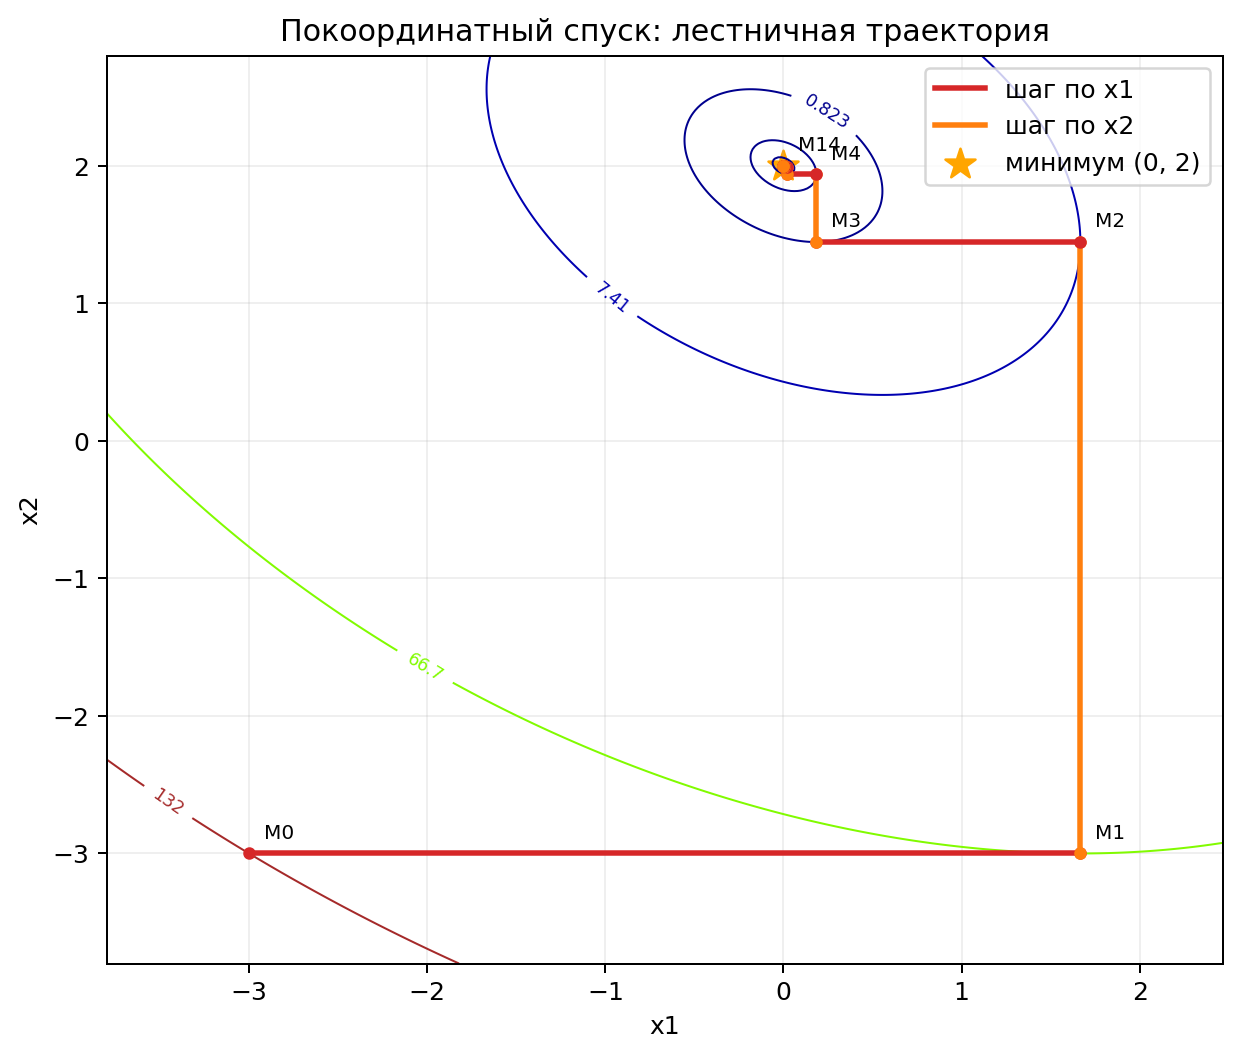
\includegraphics[width=0.82\textwidth]{dz2_coordinate_descent.png}
  \caption{Покоординатный спуск: лестничная траектория параллельно координатным осям.}
\end{figure}

\begin{figure}[H]
  \centering
  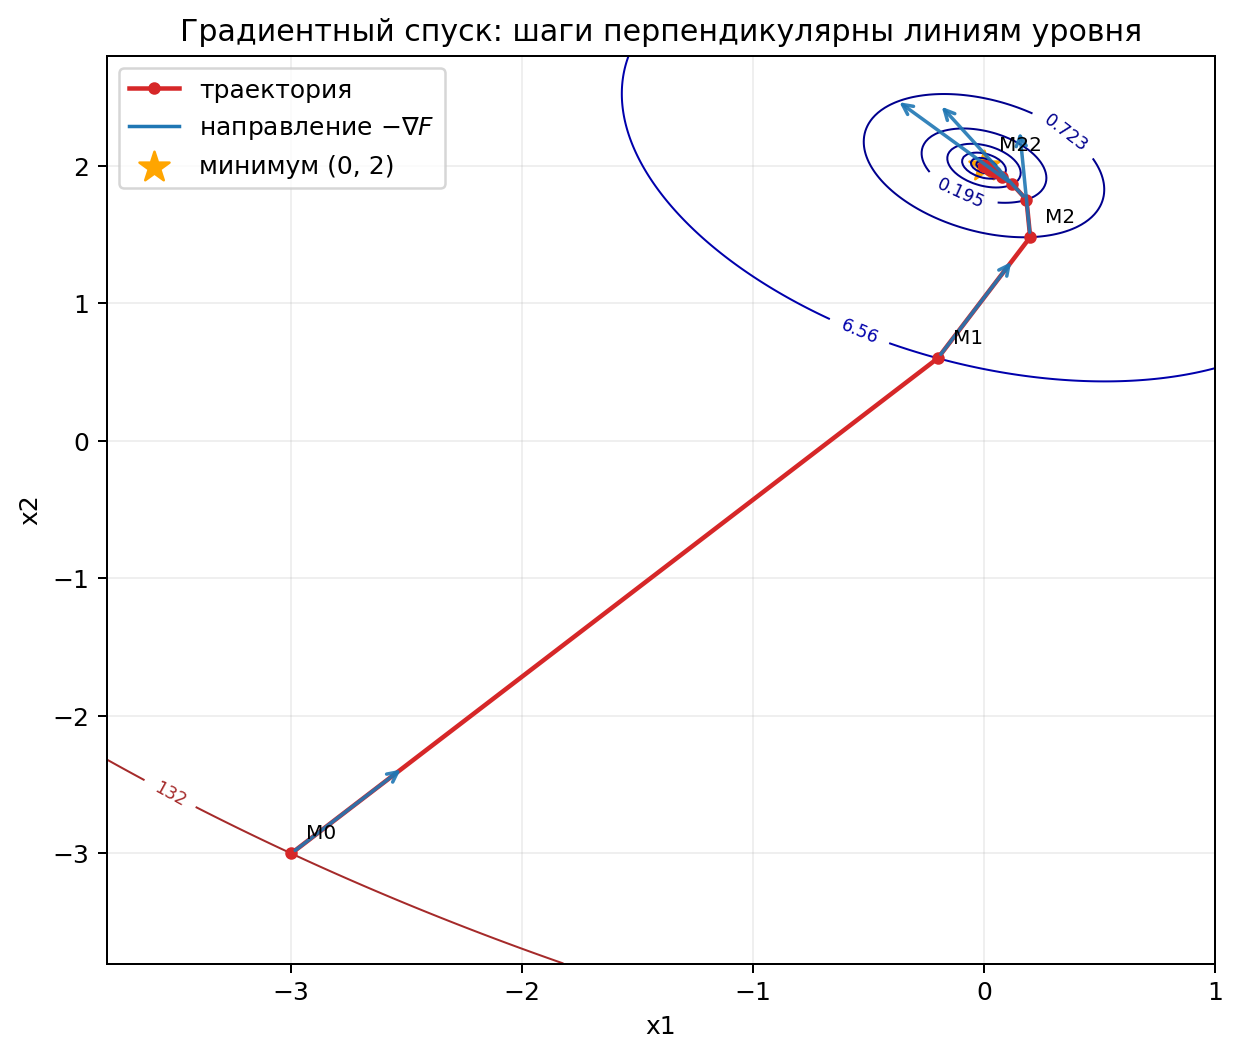
\includegraphics[width=0.82\textwidth]{dz2_gradient_descent.png}
  \caption{Градиентный спуск: шаги идут по антиградиенту, перпендикулярно линиям уровня.}
\end{figure}

\begin{figure}[H]
  \centering
  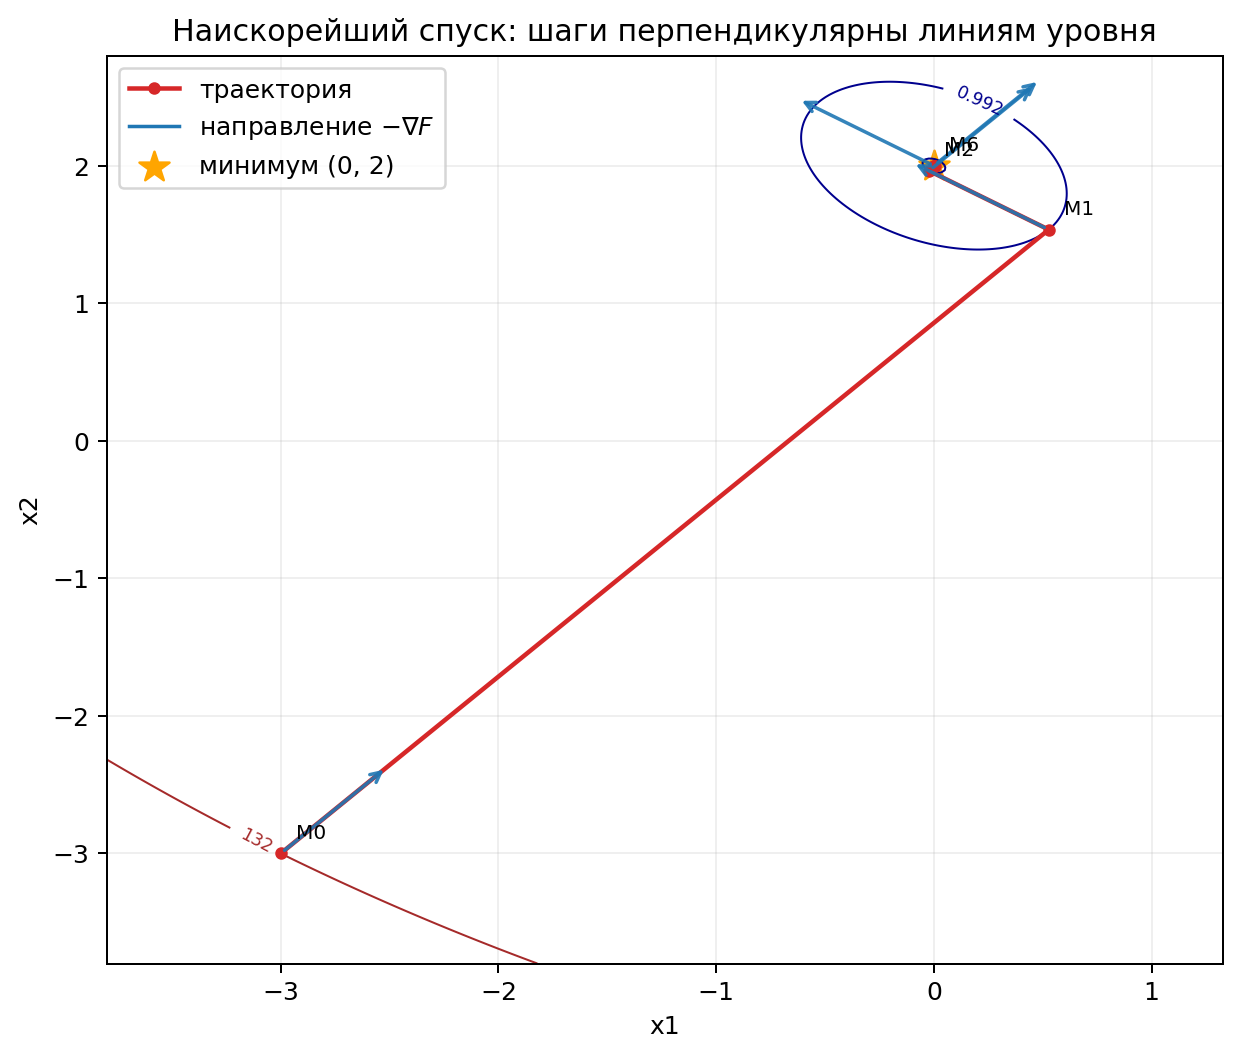
\includegraphics[width=0.82\textwidth]{dz2_steepest_descent.png}
  \caption{Наискорейший спуск: направление антиградиента и точный выбор шага.}
\end{figure}

\section{ДЗ №2.2. Метод Ньютона}

\subsection{Постановка задачи}

Для варианта 9 задана функция
\begin{equation}
  z(x,y)=x^3-6x^2+9x+y^3-11y^2+39y-49,
\end{equation}
начальная точка:
\begin{equation}
  (x_0,y_0)=(2.5,4.5).
\end{equation}

Градиент и матрица Гессе:
\begin{equation}
  \nabla z(x,y)=
  \begin{pmatrix}
    3x^2-12x+9\\
    3y^2-22y+39
  \end{pmatrix},
  \qquad
  H(x,y)=
  \begin{pmatrix}
    6x-12 & 0\\
    0 & 6y-22
  \end{pmatrix}.
\end{equation}

\subsection{Аналитическое решение и классификация стационарных точек}

Стационарные точки находятся из системы:
\begin{equation}
  3x^2-12x+9=0, \qquad 3y^2-22y+39=0.
\end{equation}
Отсюда:
\begin{equation}
  x\in\{1,3\}, \qquad y\in\left\{3,\frac{13}{3}\right\}.
\end{equation}

\begin{table}[H]
\centering
\caption{Классификация стационарных точек функции $z$}
\begin{tabular}{cccl}
\toprule
Точка & $z(x,y)$ & Собственные значения $H$ & Тип \\
\midrule
$(1,3)$ & 0.000000 & $(-6,-4)$ & локальный максимум \\
$(1,13/3)$ & -1.185185 & $(-6,4)$ & седловая точка \\
$(3,3)$ & -4.000000 & $(6,-4)$ & седловая точка \\
$(3,13/3)$ & -5.185185 & $(6,4)$ & локальный минимум \\
\bottomrule
\end{tabular}
\end{table}

\subsection{Численное решение методом Ньютона}

Формула метода Ньютона:
\begin{equation}
  X_{k+1}=X_k-H(X_k)^{-1}\nabla z(X_k).
\end{equation}
В программе обратная матрица считается явно:
\begin{equation}
  H^{-1}(X_k)=\text{\texttt{np.linalg.inv(H)}}, \qquad
  s_k=H^{-1}(X_k)\nabla z(X_k), \qquad
  X_{k+1}=X_k-s_k.
\end{equation}

Рассмотрим первый шаг подробно, как в образце отчета. Начальная точка:
\begin{equation}
  X_0=\begin{pmatrix}2.5\\4.5\end{pmatrix}.
\end{equation}
Градиент в начальной точке:
\begin{equation}
  \nabla z(X_0)=
  \begin{pmatrix}
    3\cdot 2.5^2-12\cdot 2.5+9\\
    3\cdot 4.5^2-22\cdot 4.5+39
  \end{pmatrix}
  =
  \begin{pmatrix}
    -2.25\\
    0.75
  \end{pmatrix}.
\end{equation}
Матрица Гессе и обратная матрица:
\begin{equation}
  H(X_0)=
  \begin{pmatrix}
    6\cdot 2.5-12 & 0\\
    0 & 6\cdot 4.5-22
  \end{pmatrix}
  =
  \begin{pmatrix}
    3 & 0\\
    0 & 5
  \end{pmatrix},
  \qquad
  H(X_0)^{-1}=
  \begin{pmatrix}
    \frac{1}{3} & 0\\
    0 & \frac{1}{5}
  \end{pmatrix}.
\end{equation}
Шаг Ньютона:
\begin{equation}
  s_0=H(X_0)^{-1}\nabla z(X_0)=
  \begin{pmatrix}
    \frac{1}{3} & 0\\
    0 & \frac{1}{5}
  \end{pmatrix}
  \begin{pmatrix}
    -2.25\\
    0.75
  \end{pmatrix}
  =
  \begin{pmatrix}
    -0.75\\
    0.15
  \end{pmatrix}.
\end{equation}
Новое приближение:
\begin{equation}
  X_1=X_0-s_0=
  \begin{pmatrix}2.5\\4.5\end{pmatrix}
  -
  \begin{pmatrix}-0.75\\0.15\end{pmatrix}
  =
  \begin{pmatrix}3.25\\4.35\end{pmatrix}.
\end{equation}
Критерий останова: $\|\nabla z(X_k)\|<10^{-4}$.

\begin{table}[H]
\centering
\caption{Итерации метода Ньютона}
\begin{tabular}{ccccc}
\toprule
$k$ & $(x_k,y_k)$ & $z(x_k,y_k)$ & $\nabla z(x_k,y_k)$ & $\|\nabla z\|$ \\
\midrule
0 & $(2.500000,4.500000)$ & -4.500000 & $(-2.250000,0.750000)$ & 2.371708 \\
1 & $(3.250000,4.350000)$ & -4.981500 & $(1.687500,0.067500)$ & 1.688849 \\
2 & $(3.025000,4.333537)$ & -5.183294 & $(0.151875,0.000813)$ & 0.151877 \\
3 & $(3.000305,4.333333)$ & -5.185185 & $(0.001830,0.000000)$ & 0.001830 \\
4 & $(3.000000,4.333333)$ & -5.185185 & $(0.000000,0.000000)$ & $2.79\cdot 10^{-7}$ \\
\bottomrule
\end{tabular}
\end{table}

Итоговая точка:
\begin{equation}
  \boxed{(x^*,y^*)\approx\left(3,\frac{13}{3}\right)=(3,4.333333)},
  \qquad
  \boxed{z(x^*,y^*)\approx -5.185185}.
\end{equation}

Это локальный минимум, так как в этой точке $H=\mathrm{diag}(6,4)$ положительно определена.

\begin{figure}[H]
  \centering
  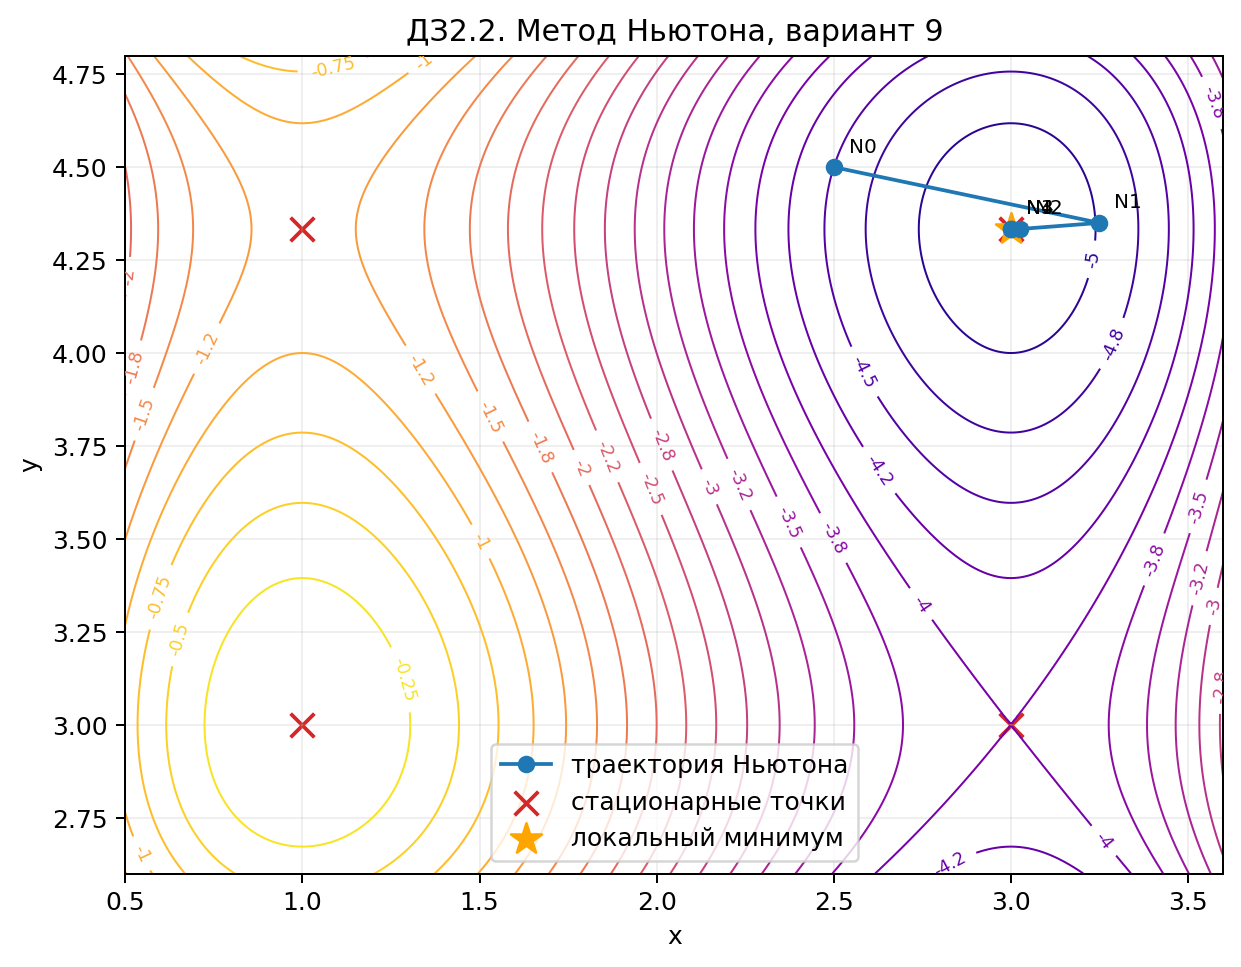
\includegraphics[width=0.82\textwidth]{dz2_newton_path.png}
  \caption{Траектория метода Ньютона и стационарные точки функции $z(x,y)$.}
\end{figure}

\section{ДЗ №2.3. Объектная модель задачи минимизации}

\subsection{Постановка объектной модели}

В программной реализации задача разбита на сущности:
\begin{itemize}
  \item \texttt{Objective2D} --- абстрактная целевая функция двух переменных;
  \item \texttt{Variant9Quadratic} --- конкретная квадратичная функция варианта 9;
  \item \texttt{Optimizer2D} --- абстрактный оптимизатор;
  \item \texttt{CoordinateDescent}, \texttt{GradientDescent}, \texttt{SteepestDescent} --- конкретные методы оптимизации;
  \item \texttt{OptimizationResult} --- объект результата, содержащий путь, значения функции и нормы градиента.
\end{itemize}

Использованные отношения:
\begin{itemize}
  \item наследование: конкретные методы наследуются от \texttt{Optimizer2D};
  \item композиция: оптимизатор содержит целевую функцию;
  \item агрегация: оптимизатор накапливает список точек траектории;
  \item использование: методы вызывают \texttt{value}, \texttt{gradient}, \texttt{hessian}.
\end{itemize}

\begin{figure}[H]
  \centering
  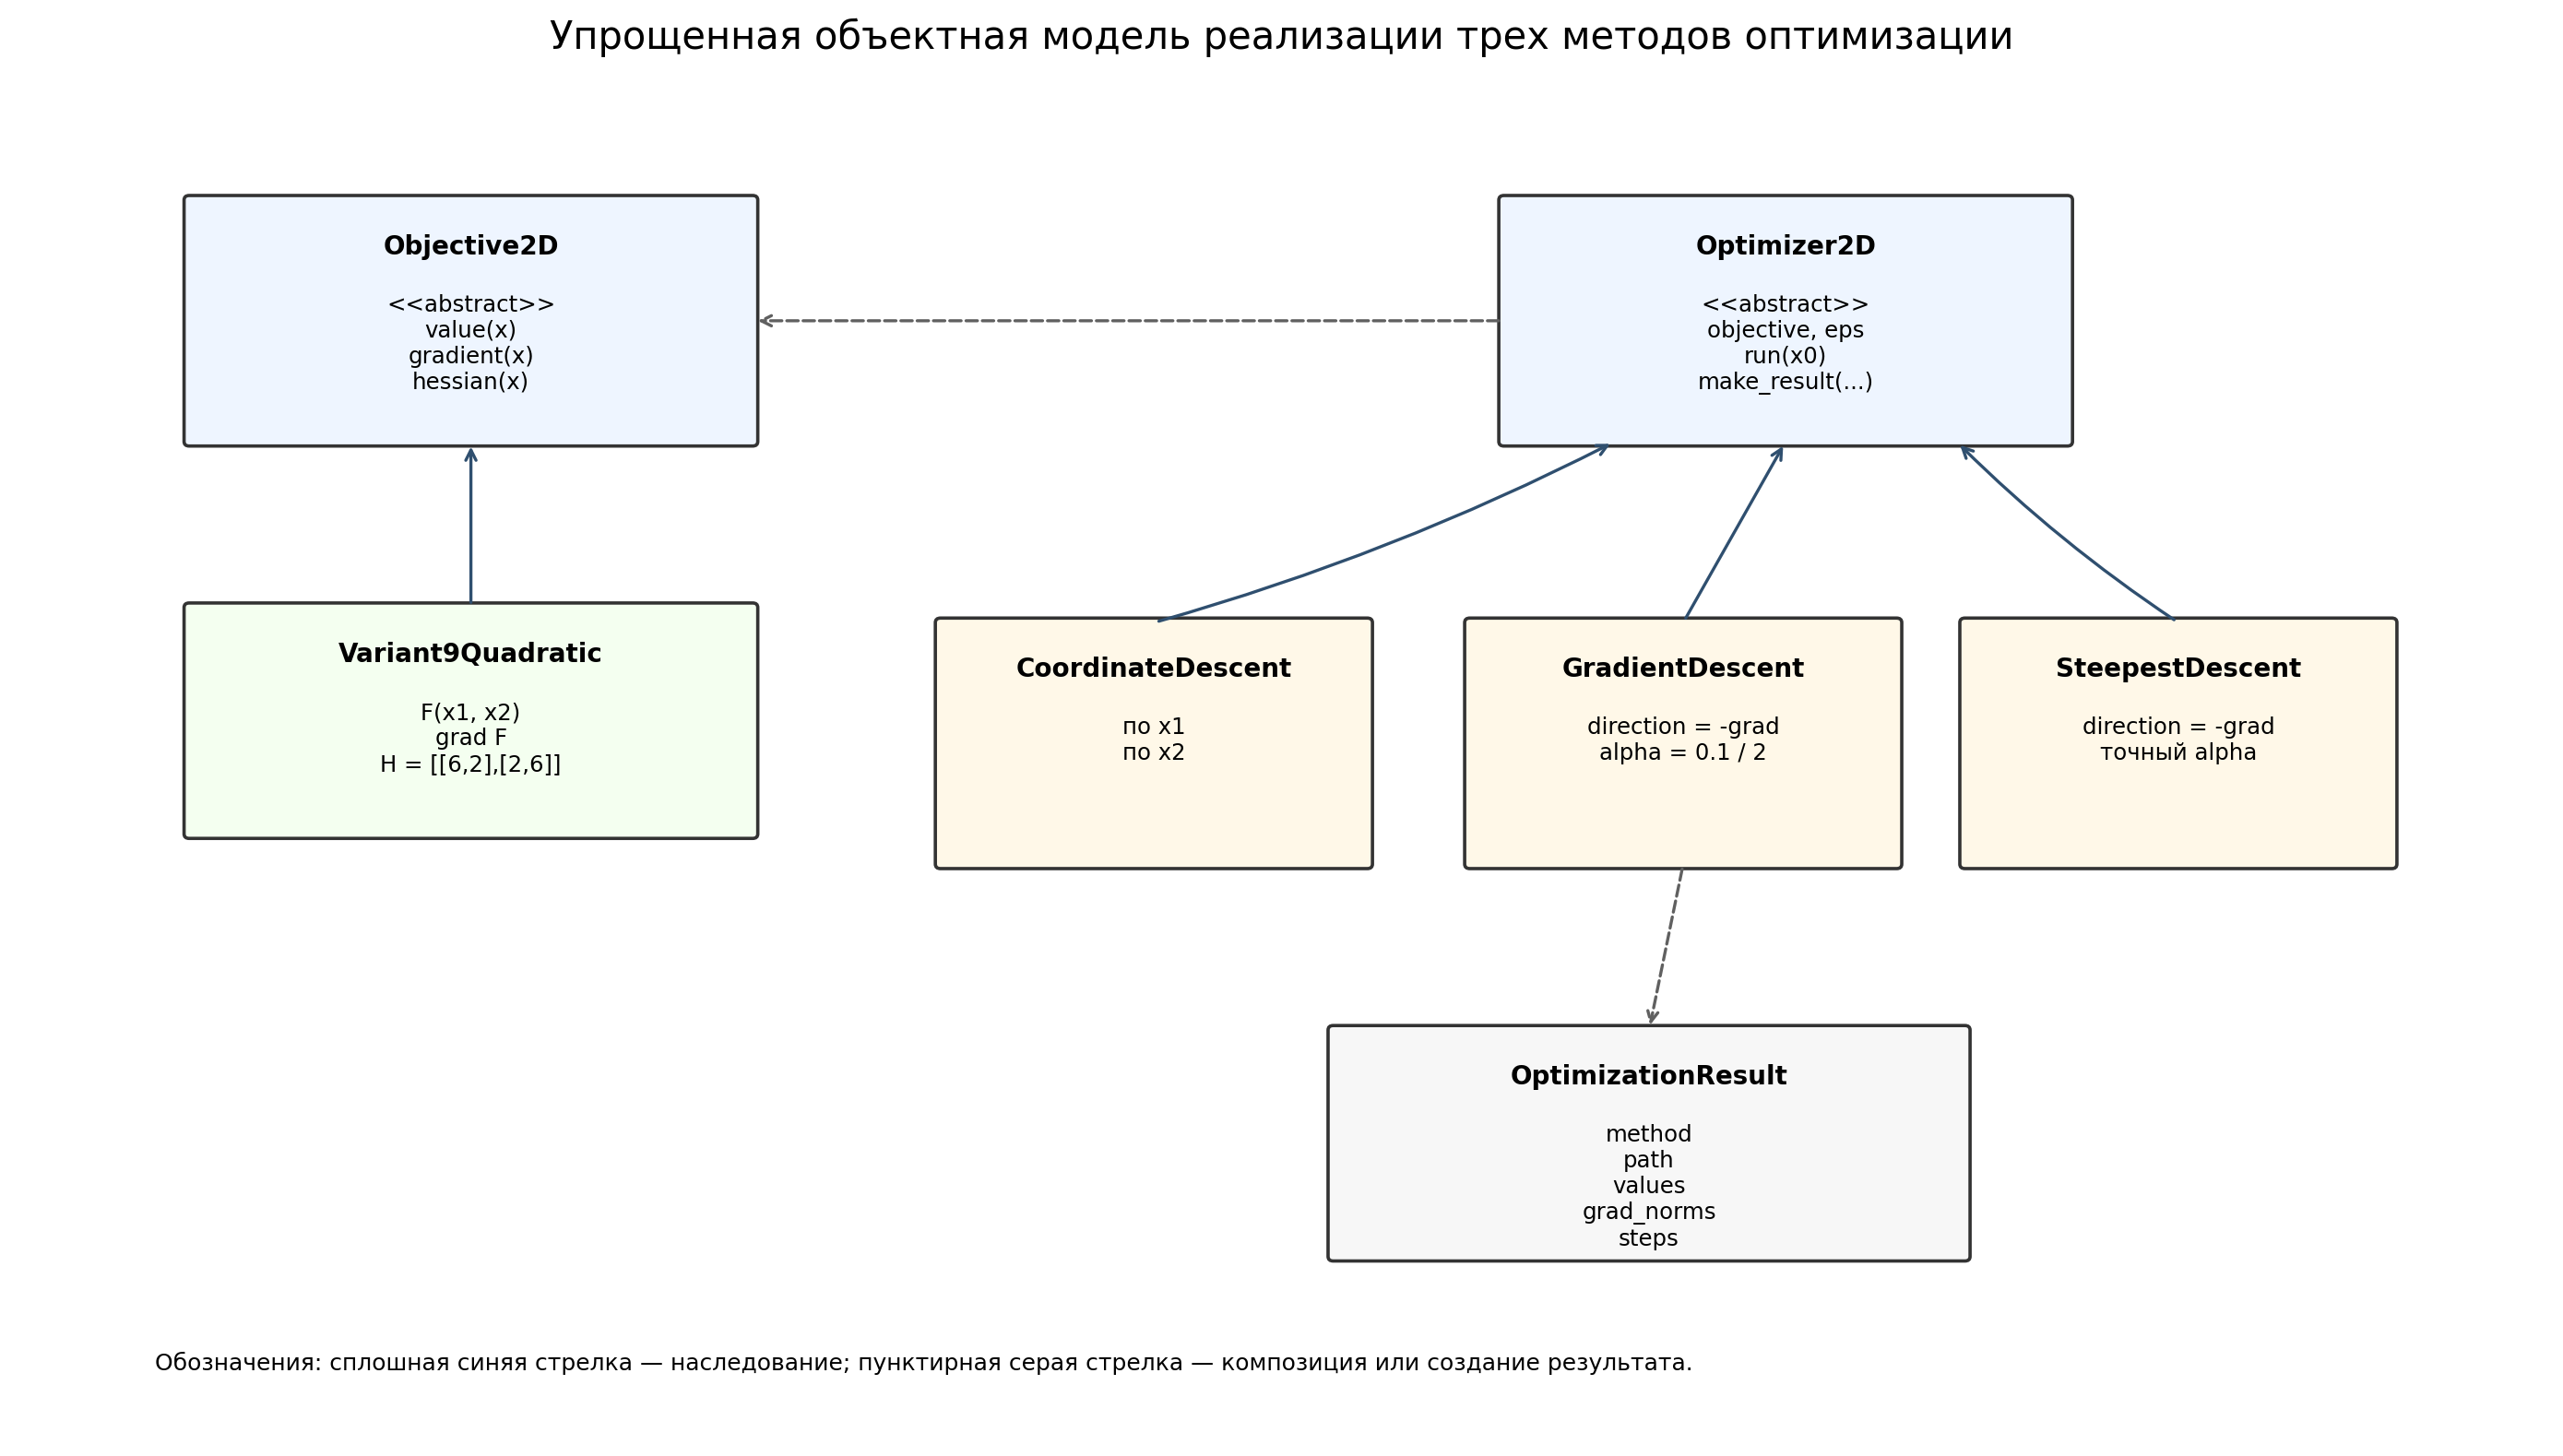
\includegraphics[width=\textwidth]{dz2_object_model.png}
  \caption{Объектная модель реализации трех методов оптимизации.}
\end{figure}

\subsection{Связь модели с кодом}

Код объектной модели находится в файле \texttt{dz2\_3\_object\_model.py}. Все три метода запускаются через единый интерфейс \texttt{run(x0)} и возвращают объект \texttt{OptimizationResult}. Благодаря этому построение графиков не зависит от конкретного метода: визуализатор получает только траекторию, значения функции и название метода.

\section{Вывод}

В ДЗ №1 методом кубической аппроксимации найден минимум функции варианта 9:
\[
  x_{\min}\approx 1.841097, \qquad f(x_{\min})\approx -6.001533.
\]

В ДЗ №2 для квадратичной функции варианта 9 все три метода из ЛР4 сошлись к единственному глобальному минимуму:
\[
  (x_1^*,x_2^*)=(0,2), \qquad F(x^*)=0.
\]

Для функции из ДЗ2.2 аналитически классифицированы все стационарные точки, а метод Ньютона из начальной точки $(2.5,4.5)$ сошелся к локальному минимуму:
\[
  (x^*,y^*)=\left(3,\frac{13}{3}\right), \qquad z(x^*,y^*)=-\frac{140}{27}\approx -5.185185.
\]

\end{document}
